%%%%%%%%%%%%%%%%%%%%%%%%%%%%%%%%%%%%%%%%%%%%%%%%%%%%%%%%%%%%%%%%%
%%% %
%%% % weiiszablon.tex
%%% % The Faculty of Electrical and Computer Engineering
%%% % Rzeszow University Of Technology diploma thesis Template
%%% % Szablon pracy dyplomowej Wydziału Elektrotechniki 
%%% % i Informatyki PRz
%%% % January, 2024
%%%%%%%%%%%%%%%%%%%%%%%%%%%%%%%%%%%%%%%%%%%%%%%%%%%%%%%%%%%%%%%%%

\documentclass[12pt,twoside]{article}

\usepackage{weiiszablon}

\author{Michał Bazan}

% np. EF-123456, EN-654321, ...
\studentID{EF-163881}

\title{Porównanie algorytmów nawigacyjnych}
\titleEN{Comparison of navigation algorithms}


%%% wybierz rodzaj pracy wpisując jeden z poniższych numerów: ...
% 1 = inżynierska	% BSc
% 2 = magisterska	% MSc
% 3 = doktorska		% PhD
% 4 = praca inżynierska
%%% na miejsce zera w linijce poniżej
\newcommand{\rodzajPracyNo}{2}


%%% promotor
\supervisor{dr inż. Dariusz Rzońca}
%% przykład: dr hab. inż. Józef Nowak, prof. PRz

%%% promotor ze stopniami naukowymi po angielsku
\supervisorEN{Dariusz Rzońca, dr. engineer}

\abstract{Praca koncentruje się na badaniu wybranych algorytmów nawigacyjnych oraz metod optymalizacji nastaw regulatorów PID z wykorzystaniem zbudowanego robota mobilnego, który został skonstruowany zgodnie z procedurami ASPICE. Celem jest ocena dokładności, szybkości wyznaczania trasy oraz ogólnej wydajności tych algorytmów. Analiza wyników pozwoli wyciągnąć wnioski dotyczące skuteczności i efektywności badanych algorytmów nawigacyjnych. Dzięki zastosowaniu standardów ASPICE zapewniona została wysoka jakość procesu budowy robota, co umożliwia rzetelne i wiarygodne badania nad jego funkcjonalnością i algorytmami nawigacyjnymi.}
\abstractEN{
The work focuses on the study of selected navigation algorithms and methods for optimising PID controller settings using a built mobile robot that has been constructed according to ASPICE procedures. The aim is to evaluate the accuracy, routing speed and overall performance of these algorithms. Analysis of the results will allow conclusions to be drawn regarding the effectiveness and efficiency of the navigation algorithms studied. Through the use of ASPICE standards, the high quality of the robot construction process is ensured, enabling reliable and credible research into its functionality and navigation algorithms.}

\keywords{Algorytmy nawigacyjne, Robot mobilny, Inżynieria, ASPICE, Machine Learning}
\keywordsEN{Navigation algorithms, Mobile robot, Engineering, ASPICE, Machine Learning}


\begin{document}

% strona tytułowa
\maketitle

\blankpage

% spis treści
\tableofcontents

\clearpage
\blankpage


\section*{Wykaz symboli, oznaczeń i skrótów}


\section{Wstęp}
W dzisiejszych czasach, wraz z dynamicznym rozwojem technologii mobilnych, algorytmy nawigacyjne i uczenia maszynowego \cite{deepLearning} odgrywają kluczową rolę w różnorodnych aplikacjach, począwszy od systemów nawigacji w samochodach po autonomiczne roboty poruszające się w różnych środowiskach. Biorąc pod uwagę aktualność tych zagadnień i rosnące zapotrzebowanie, zdecydowano o przeprowadzeniu badań dotyczących systemów nawigacyjnych.
   
Celem tej pracy jest zbadanie heurystycznych metod \cite{genetics} optymalizazcji regulatorów PID oraz porównanie wybranych algorytmów pod kątem kryteriów takich jak dokładność wyznaczania trasy oraz wydajność obliczeniowa w różnych warunkach terenowych.  

Zakres pracy obejmuje dwie części:
\begin{enumerate}[label=\alph*), leftmargin=1.25cm]
	\item część inżynierska - wykonanie robota mobilnego, implementacja systemu wbudowanego oraz implementacja oprogramowania sterującego robotem poprzez dostępny interfejs,
	\item część badawcza - badanie algorytmów uczenia maszynowego do optymalizacji nastaw regulatorów PID oraz porównanie wybranych algorytmów nawigacyjnych. 
\end{enumerate}

Zastosowanie standardu ASPICE \cite{SPICE} zapewnia wysoką jakość procesu budowy robota oraz implementacji oprogramowania co pozwola na przeprowadzenie rzetelnych badań i wyciągnięcie wiarygodnych wniosków.

W dalszej części pracy szczegółowo omówione zostaną poszczególne etapy realizacji każdego z tych komponentów, prezentując zarówno teoretyczne założenia, jak i praktyczne wyniki osiągnięte w ramach projektu.

W następnych rozdziałach pracy przedstawiono szczegółowy opis inżynierskiej części projektu oraz wyniki przeprowadzonych badań. W rozdziale poświęconym inżynierskiej części projektu omówiono budowę robota, jego system operacyjny oraz prostą stację operatorską, które stanowią podstawę do realizacji badań algorytmicznych. Następnie, w rozdziale dotyczącym badanych algorytmów, zaprezentowano teoretyczne i praktyczne aspekty algorytmu genetycznego, algorytmów nawigacyjnych statycznych oraz dynamicznych. Kolejny rozdział skupia się na opisie przeprowadzonych badań, w których dokonano optymalizacji nastaw regulatora PID oraz przeprowadzono porównanie skuteczności algorytmów nawigacyjnych. Te szczegółowe analizy mają na celu ocenę wydajności poszczególnych rozwiązań oraz identyfikację optymalnych metod nawigacyjnych dla zbudowanego robota.

\section{Inżynierska część projektu}

W tym rozdziale przedstawiono kompleksowy opis prac związanych z implementacją oraz funkcjonowaniem robota. Niniejszy rozdział stanowi szczegółowe omówienie trzech kluczowych elementów projektu, które skupiały się na budowie fizycznej robota zgodnie z procedurami SPICE, implementacji oprogramowania w języku C++ z uwzględnieniem unit testów oraz oprogramowania do sterowania robotem. Dzięki zastosowaniu tych trzech elementów możliwe było zapewnienie nie tylko skutecznej implementacji samego robota, ale również jego oprogramowania oraz efektywnego zarządzania nim w czasie rzeczywistym.
Dokładna dokumentacja wszystkich komponentów projektu oraz testów znajduje się na repozytorium Github \cite{repo}.

\subsection{Budowa robota}

Pierwszym aspektem, który zostanie przedstawiony, jest proces budowy robota. Opisane zostaną tutaj szczegóły dotyczące wyboru komponentów oraz implementacji elektroniki sterującej.

\subsubsection{Wymagania sprzętowe}

W celu dobrania właściwych elementów do budowy robota, sformułowano niżej umieszczone wymagania wysokiego poziomu:

\begin{table}[ht]
\caption{Wymagania wysokiego poziomu HWE1}
\centering		
	\begin{tabular}{|c|p{0.7\textwidth}|}	
		\hline
		ID\_HWE1 & Opis \\
		\hline
		HWE\_1\_010 & Sprzęt powinien wspierać obsługę czujników odległości. \\
		\hline
		HWE\_1\_020 & Kontroler powinien udostępniać moduł WiFi. \\
		\hline 
		HWE\_1\_030 & Robot powinien być wyposażony w szczotkowe silniki DC z enkoderami.\\
		\hline
		HWE\_1\_040 & Sprzęt powinien wspierać obsługę enkoderów. \\
		\hline
		HWE\_1\_060 & Sprzęt powinien mieć zaimplementowany odpowiedni system dystrybucji zasilania. \\
		\hline

	\end{tabular}	
	
\label{Tab:HWE1}
\end{table}	

\newpage

Na podstawie wyżej ukazanych, sformułowano następujące wymagania niskiego poziomu:


\begin{table}[ht]
\caption{Wymagania niskiego poziomu HWE2}
\centering
\begin{tabular}{|c|p{0.7\textwidth}|}	
    \hline
    ID\_HWE2 & Opis \\
    \hline
    HWE\_2\_010 & Wszystkie interfejsy komunikacyjne powinny wspierać logikę 3V3. \\
    \hline
    HWE\_2\_020 & Mikrokontroler powinien być wyposażony w moduł WiFi. \\
    \hline 
    HWE\_2\_030 & System dystrybucji zasilania powinien zasilić logikę.\\
    \hline
    HWE\_2\_040 & System dystrybucji zasilania powinien zasilić silniki. \\
    \hline
    HWE\_2\_060 & Czujnik odległości powinien mieć zakres pomiarowy wynoszący conajmniej 200 cm. \\
    \hline
    HWE\_2\_070 & Czujniki odległości powinny udostępniać interfejs komunikacyjny kompatybilny z interfejsami mikrokontrolera. \\
    \hline
\end{tabular}
\label{Tab:HWE2}
\end{table}
	

\begin{figure}[ht]%
 \centering%
 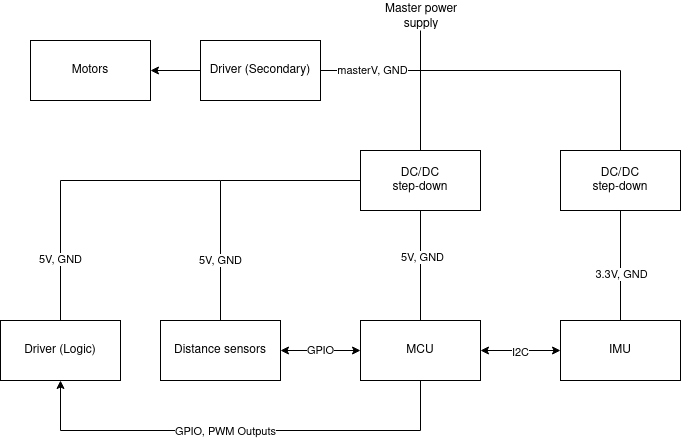
\includegraphics[width=12cm]{figures/engHW/robotblock.png}%
 \caption{Schemat blokowy sprzętu}%
 \label{Fig:schemat}%
\end{figure}

Wyżej załączona figura \ref{Fig:schemat} ukazuje schemat blokowy utworzony na podstawie wcześniej zdefiniowanych wymagań sprzętowych. Wskazuje, jakie interfejsy i poziomy napięć zasilania zostały wykorzystane pomiędzy poszczególnymi blokami. Sprzęt zdefiniowany w ten sposób i zbiór wymagań stawianych przed urządzeniem zezwolił na dobranie właściwych komponentów. 

\newpage

\subsubsection{Schemat elektryczny}
Niniejsza sekcja skupia się na wyjaśnieniu schematu elektrycznego robota. 
Na podstawie umieszczonych w poprzedniej sekcji wymagań dokonano wyboru komponentów, które zostały wykorzystane w projekcie, ale dokładny opis elementów został umieszczony w dokumentacji tej części projektu na repozytorium Github \cite{repo}.\\
\newline
W celu ułatwienia procesu implementacji i zmitygowaniu potencjalnych błędów, schemat elektryczny został podzielony na bloki zgodnie z podziałem ukazanym na rysunku \ref{Fig:schemat}.



\begin{figure}[ht]%
 \centering%
 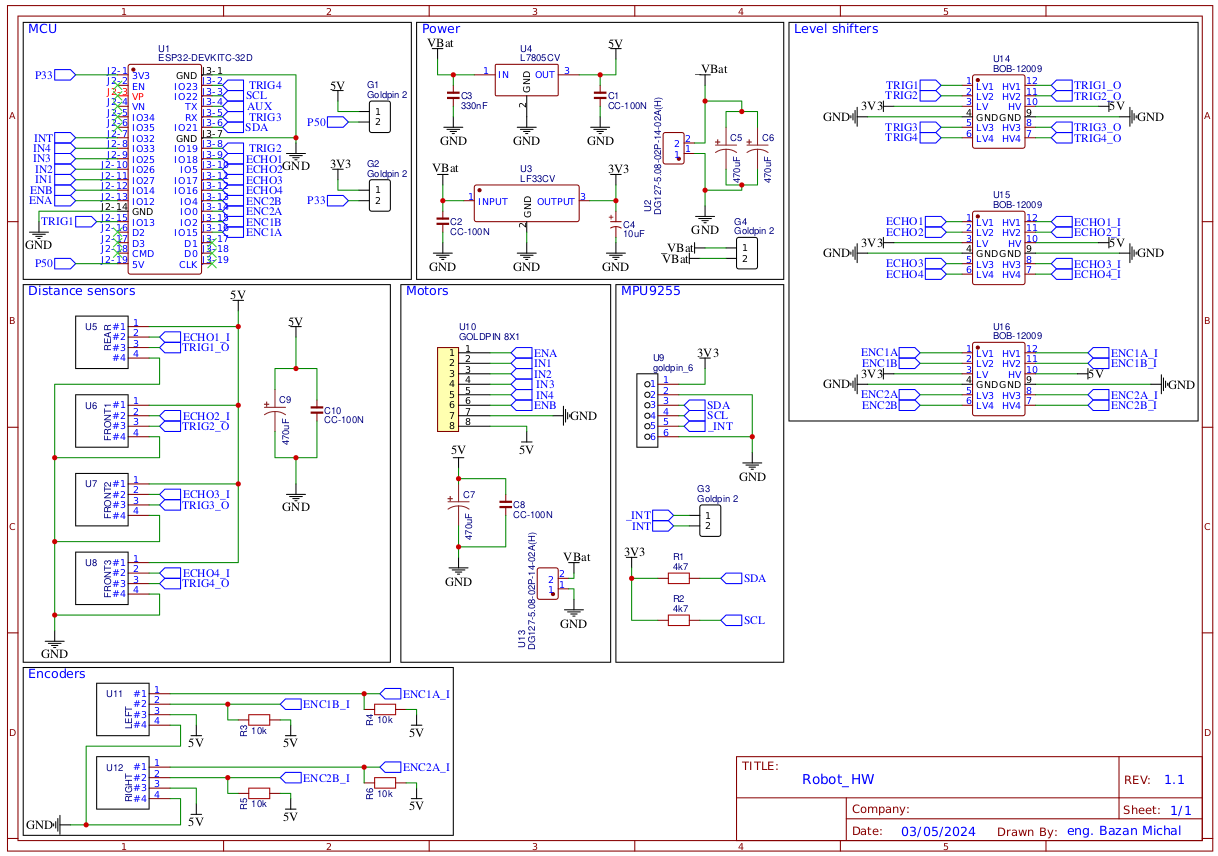
\includegraphics[width=12cm]{figures/engHW/robotschem.png}%
 \caption{Schemat elektryczny}%
 \label{Fig:elektryczny}%
\end{figure}

Wyżej umieszczona ilustracja \ref{Fig:elektryczny} ukazuje połączenia pomiędzy blokami schematu:

\begin{enumerate}[label=\alph*), leftmargin=1.25cm]
	\item MCU - blok definiuje wejścia i wyjścia sterujące oraz połączenia interfejsów komunikacyjnych,
	\item Power - sekcja odpowiedzialna za dystrybucję zasilania,
	\item Level shifters - konwertery poziomów logicznych, które zapewniają kompatybilność poziomów sygnałów elektrycznych,
	\item Distance sensors - blok definiuje połączenia pomiędzy mikrokontrolerem i czujnikami odległości,
	\item Motors - sekcja ukazuje sygnały sterujące silnikami,
	\item MPU9255 - blok został zaimplementowany, ale nie jest wykorzystywany,
	\item Encoders - ta sekcja ukazuje sygnały wyjściowe z enkoderów.
\end{enumerate}

\subsubsection{Testy}
Testowanie tej części projektu polegało głównie na weryfikacji założeń i projektu płytki, dlatego aspekt ten nie został poruszony w tej sekcji. Szczegółowa dokumentacja znajduje się w zdalnym repozytorium \cite{repo}. 

\newpage

\subsection{System operacyjny robota}

Ta sekcja skupia się na implementacji oprogramowania w języku C++, obejmującej zarówno projektowanie jak i implementacja funkcjonalności.

\subsubsection{Wymagania dotyczące oprogramowania}

Na podstawie wcześniej omówionych wymagań sprzętowych oraz celów tego projektu, sformułowano następujące wymagania wysokiego poziomu:

\begin{enumerate}[label=\alph*), leftmargin=1.25cm]
	\item Oprogramowanie powinno odczytywać sensory periodycznie,
	\item Interfejs WiFi powinien być wykorzystany do komunikacji z oprogramowaniem sterującym,
	\item Oprogramowanie powinno udostępniać interfejs do sterowania silnikami,
	\item Komunikacja powinna wykorzystywać prosty protokół komunikacyjny do wymiany danych pomiędzy robotem a oprogramowaniem sterującym,
	\item Oprogramowanie powinno implementować algorytm wyznaczający odometrię.
\end{enumerate}




\subsubsection{Implementacja}

\subsubsection{Obsługiwane komendy}

\subsection{Sterowanie robotem}

Kolejnym istotnym zagadnieniem będzie omówienie wykorzystania ROS2 oraz technologii Docker w kontekście sterowania robotem. Przedstawione zostaną tutaj zarówno zalety jak i wyzwania związane z integracją tych narzędzi.

\section{Badane algorytmy}

\subsection{Algorytm genetyczny}
\subsection{Uczenie ze wzmocnieniem}
\subsection{Algorytmy nawigacyjne}


\section{Badania}
\subsection{Optymalizacja nastaw regulatora PID prędkości obrotowej}
\subsection{Optymalizacja nastaw regulatora położenia i orientacji}
\subsection{Porównanie algorytmów nawigacyjnych w terenie bez przeszkód}
\subsection{Porównanie algorytmów nawigacyjnych w terenie z przeszkodami}

\section{Podsumowanie i wnioski końcowe}


\section*{Załączniki}



\clearpage

\addcontentsline{toc}{section}{Literatura}

\begin{thebibliography}{5}
\bibitem{repo} https://github.com/DevxMike/master\_degree
\bibitem{deepLearning} Francois Chollet: Deep Learning. Praca z językiem Python i biblioteką Keras. Helion 2019
\bibitem{RL} Paweł Cichosz: Systemy uczące się. WNT 2007 
\bibitem{genetics}  Riccardo Poli, William B. Langdon, Nicholas F. McPhee, John R. Koza: A Field Guide to Genetic Programming. Lulu Enterprises Uk Ltd 2008
\bibitem{SPICE} https://mfiles.pl/pl/index.php/Automotive\_SPICE
\end{thebibliography}

\clearpage

\makesummary

\end{document} 
